{\LARGE Output:}

Does the pitch of the tone that you hear increase with each increase in the frequency $\Omega_0$? If not, can you explain this behavior?

The Pitch of the tone increase to the highest frequency at $\omega_0 = 4000$ and then it decreases in pitch. This Can be observed with the Matlab script which was created as a function(Code 7.1-6). 

$>>$ Part1Code\_F(3500,0)\\
$>>$ Part1Code\_F(4000,0)\\
$>>$ Part1Code\_F(4500,0)\\
$>>$ Part1Code\_F(5000,0)\\
$>>$ Part1Code\_F(5500,0)


\begin{figure}[!htbp]
  \centering
    \includegraphics[width=0.7\textwidth]{Part1/Output/Figures/proj71PartF-3500.eps}
  \caption{Output for 7.1 Part F | $\Omega_0 = 2\pi(3500)$ }
\end{figure}

\begin{figure}[!htbp]
  \centering
    \includegraphics[width=0.7\textwidth]{Part1/Output/Figures/proj71PartF-4000.eps}
  \caption{Output for 7.1 Part F | $\Omega_0 = 2\pi(4000)$ }
\end{figure}

\begin{figure}[!htbp]
  \centering
    \includegraphics[width=0.7\textwidth]{Part1/Output/Figures/proj71PartF-4500.eps}
  \caption{Output for 7.1 Part F | $\Omega_0 = 2\pi(4500)$ }
\end{figure}

\begin{figure}[!htbp]
  \centering
    \includegraphics[width=0.7\textwidth]{Part1/Output/Figures/proj71PartF-5000.eps}
  \caption{Output for 7.1 Part F | $\Omega_0 = 2\pi(5000)$ }
\end{figure}

\begin{figure}[!htbp]
  \centering
    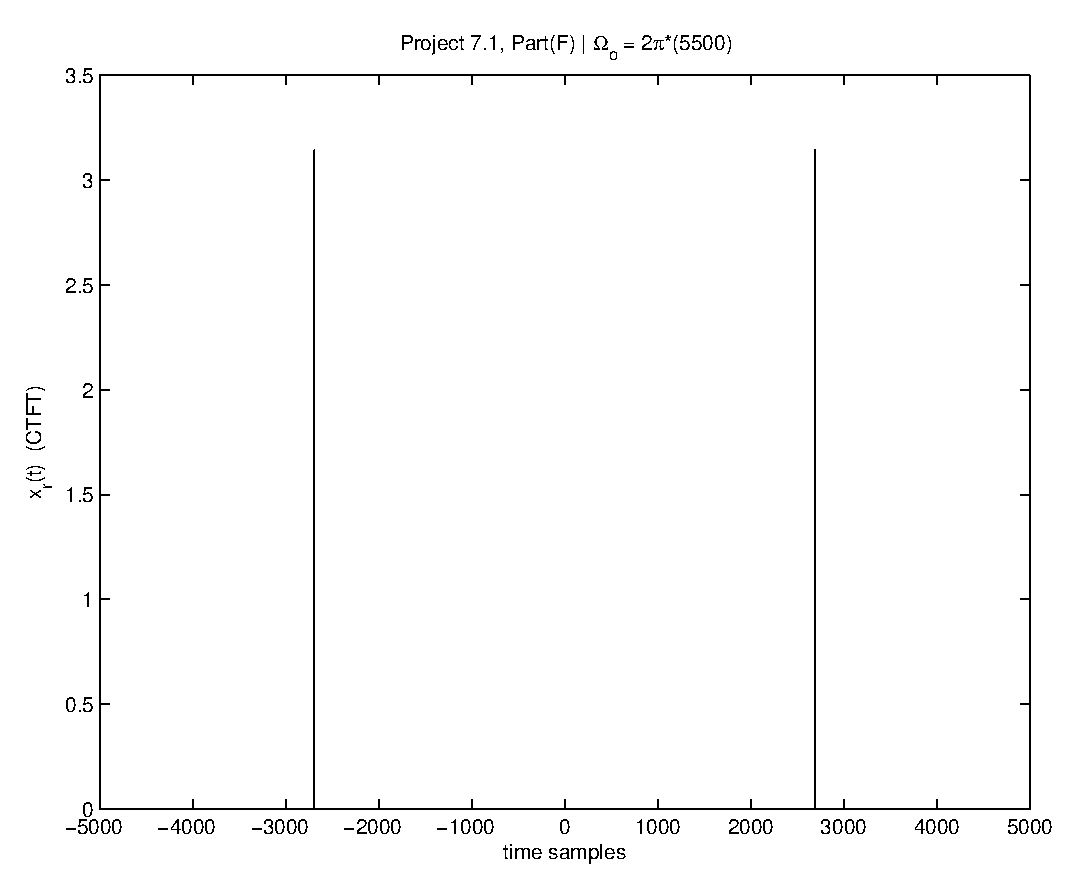
\includegraphics[width=0.7\textwidth]{Part1/Output/Figures/proj71PartF-5500.eps}
  \caption{Output for 7.1 Part F | $\Omega_0 = 2\pi(5500)$ }
\end{figure}


\pagebreak
